\chapter{Cronometro}

\section{Cronometro}
\paragraph{Traccia}
Progettare, implementare in VHDL e testare mediante simulazione un cronometro, in grado di scandire secondi, minuti e ore a partire da una base dei tempi prefissata (es. si consideri il clock a disposizione sulla board). Il progetto deve prevedere la possibilità di inizializzare il cronometro con un valore iniziale, sempre espresso in termini di ore, minuti e secondi, mediante un opportuno ingresso di set, e deve prevedere un ingresso di \textit{reset} per azzerare il tempo.
Il componente deve essere realizzato utilizzando un approccio strutturale, collegando opportunamente dei contatori secondo uno schema a scelta. 

\subsection{Architettura}

Il sistema, realizzato con un approccio strutturale, comprende quattro componenti principali. In particolare, sono stati adibiti tre contatori per il conteggio dei secondi, minuti e ore, mentre il quarto componente è un divisore di frequenza. 

Le interconnessioni tra i componenti sono visibili nella seguente architettura: 
\begin{figure}[H]
    \centering
    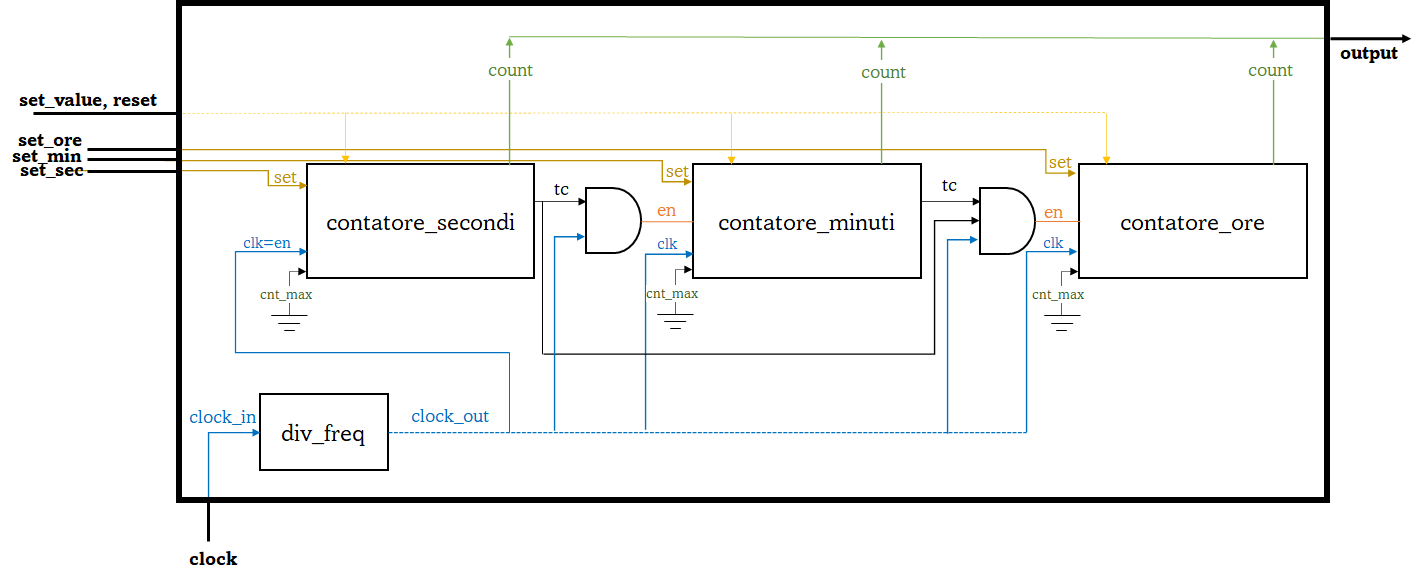
\includegraphics[width=17cm]{immagini/esercizio5/schema_5.1.png}
    \caption{Schema Cronometro}
\end{figure}

\paragraph{Contatore programmabile}
I primi tre contatori sono stati implementati a partire dallo stesso codice, tramite una \textit{entity contatore} realizzata con il costrutto \textit{generic}, al quale viene passato il valore \textit{n} che rappresenta il numero di bit necessari per effettuare il conteggio. 
Il contatore ha i seguenti input e output:
\begin{itemize}
\item \textit{cntmax}: serve per memorizzare il valore massimo del conteggio.
\item \textit{setvalue}: serve per memorizzare il valore da settare
\item \textit{clk}: segnale di clock
\item \textit{rst}: segnale di reset
\item \textit{set}: dà l’abilitazione al set al valore passato in setvalue
\item \textit{tc}: viene alzato quando si è arrivati al conteggio massimo
\item \textit{count}: valore  in uscita del conteggio corrente
\item \textit{en}: il segnale che proviene o dal clock diviso o da un altro contatore, e scandisce il momento in cui contare secondi, minuti o ore.
\end{itemize}
Il componente è stato realizzato con un unico \textit{process}, sensibile solo al \textit{clock} sul fronte di discesa, al cui interno ci sono una serie di costrutti di selezione in cascata. Inizialmente viene testata la condizione per il \textit{reset} sincrono, poi si controlla il valore di \textit{set} e nel caso è alto viene scritto nel registro il valore in input. Successivamente, se il valore di \textit{enable} è alto, si procede all'incremento del contatore,  e se si è raggiunto il valore massimo si riporta a zero e si alza l'uscita \textit{tc}. È di particolare importanza la scelta di utilizzare sia il \textit{clock} che il segnale \textit{enable}: tecnicamente si sarebbe potuto utilizzare solo il segnale di \textit{enable}, al posto del \textit{clock} normale, per abilitare i contatori in cascata (minuti e ore) , ma questo comporta che i \textit{process} si attivino ogni minuto o ogni ora. In questo modo non si sarebbe potuto  effettuare un \textit{reset} sincrono, a meno di aspettare un tempo eccessivo. L'ipotesi di usare invece un \textit{reset} asincrono è stata scartata in quanto creerebbe delle problematiche di accuratezza sull'orario misurato: se arrivasse il \textit{reset} asincrono poco prima di un nuovo \textit{clock} il secondo iniziale sarebbe contato molto prima del dovuto, come mostrato in figura.

\begin{figure}[H]
    \centering
    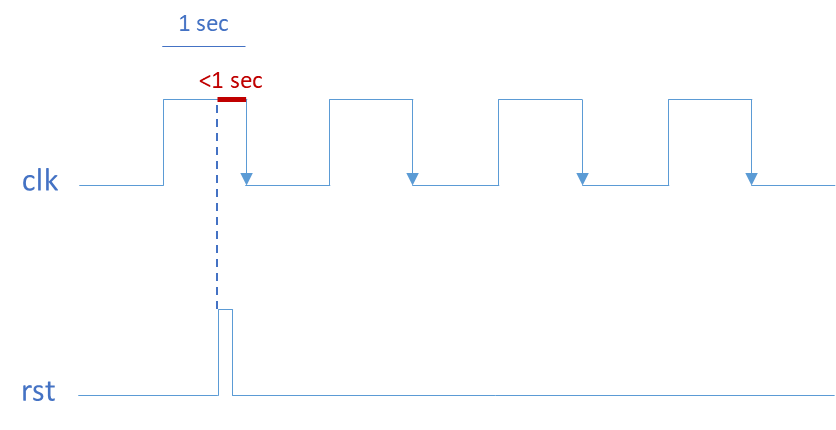
\includegraphics[width=17cm]{immagini/esercizio5/errore_reset.png}
    \caption{Reset Asincrono Errato}
\end{figure}

Di seguito il codice per l'implementazione di un contatore programmabile:
\begin{lstlisting} [language=VHDL, caption= Contatore programmabile]
library IEEE;
use IEEE.std_logic_1164.all;
use IEEE.numeric_std.all;

entity contatore is
    generic (
        n: positive
    );
    port (
        cnt_max, set_value: in std_logic_vector(n-1 downto 0);
        clk, rst, set, en: in std_logic;
        tc: out std_logic;
        count: out std_logic_vector(n-1 downto 0)
    );
end entity contatore;

architecture rtl of contatore is

begin
    proc_name: process(clk)
        variable current: unsigned(n-1 downto 0) := (others => '0');
    begin
        if falling_edge (clk) then
            if rst = '1' then
                current := (others => '0');
                tc <= '0';

            elsif set = '1' then
                current := unsigned(set_value);

            elsif en = '1' and  (unsigned(cnt_max) - 1 = current) then
                current := (others => '0');

            elsif en = '1' then
                current := current +1;
            end if;

            if(unsigned(cnt_max) - 1 = current ) then
                tc <= '1';
            else 
                tc <= '0';
            end if;
        end if;
        
        count <= std_logic_vector(current);
        
    end process proc_name;
end architecture rtl;
\end{lstlisting}

\paragraph{Divisore di frequenza}
Il divisore di frequenza è un componente necessario e serve per generare un impulso a frequenza inferiore rispetto a quella del \textit{clock} in entrata, che nel nostro caso è proprio il \textit{clock} a 100MHz della scheda.
Anche questo componente utilizza il costrutto \textit{generic} per poter essere \textit{istanziato} con diverse impostazioni. In particolare, è possibile specificare la frequenza in entrata e quella in uscita. Dopo aver inserito questi due valori viene calcolato il massimo conteggio da effettuare, in modo da alzare l'uscita una volta raggiunto il valore \textit{cnt\_max-1}. In questo caso la frequenza di uscita è stata scelta a 1Hz in modo da avere un impulso al secondo.

Il componente è stato realizzato mediante il seguente codice:
\begin{lstlisting} [language=VHDL, caption= Divisore di frequenza]
library IEEE;
use IEEE.STD_LOGIC_1164.ALL;
 
entity clock_divider is
     generic(
          clock_frequency_in : integer := 100000000;--100MHz
          clock_frequency_out : integer := 1 --1 Hz
         );
    Port ( clock_in : in  STD_LOGIC;
           reset : in STD_LOGIC;
           clock_out : out  STD_LOGIC);
end clock_divider;
 
architecture Behavioral of clock_divider is
 
signal clockfx: std_logic := '0';
constant count_max_value: integer := (clock_frequency_in/clock_frequency_out)-1;
begin
  clock_out <= clockfx;
 
    count_for_division: process(clock_in)
    variable counter: integer range 0 to count_max_value := 0;
    begin
       if rising_edge(clock_in)  then
       
        if reset = '1' then
             counter := 0;
             clockfx <= '0';
        else
          if counter = count_max_value then
              clockfx <=  '1';
              counter := 0;
           else
              clockfx <=  '0';
              counter := counter + 1;
          end if;
        end if;
       end if;
    end process;
end Behavioral;
\end{lstlisting}

\paragraph{Cronometro}
I singoli componenti analizzati fin ora sono stati collegati tra loro per realizzare il cronometro. Vengono creati tre contatori(due contano fino a 60 e uno fino a 24) e un divisore di frequenza. L'uscita del divisore (un \textit{clock} a 1 secondo) entra come \textit{enable} nel contatore dei secondi, mentre per i contatori successivi viene effettuata una \textit{AND} tra questo segnale e i segnali di uscita \textit{tc} per i minuti e le ore. In questo modo i segnali di abilitazione per scandire i minuti e le ore avranno la giusta durata, e non sarà possibile contare più volte con lo stesso fronte del segnale.
L'output totale viene calcolato concatenando le uscite dei singoli contatori in ordine.

\begin{lstlisting} [language=VHDL, caption=Cronometro]
library IEEE;
use IEEE.STD_LOGIC_1164.ALL;

entity cronometro is
    Port (
        set_value: in std_logic_vector (5 downto 0 );
        set_sec,set_min,set_ore: in std_logic;
        reset: in std_logic;
        clock: in std_logic;
        output: out std_logic_vector (16 downto 0 )
    );
end cronometro;

architecture Structural of cronometro is

    component contatore is
        generic (
            n: positive
        );
        Port (
            cnt_max, set_value: in std_logic_vector(n-1 downto 0);
            clk, rst, set, en: in std_logic;
            tc: out std_logic;
            count: out std_logic_vector(n-1 downto 0)
        );
    end component;

    component clock_divider is
        generic(
            clock_frequency_in : integer := 100000000;--100MHz
            clock_frequency_out : integer := 10000000 --10 MHz
        );
        Port ( clock_in : in  STD_LOGIC;
             reset : in STD_LOGIC;
             clock_out : out  STD_LOGIC);
    end component;

    signal s_clk:std_logic;
    signal s_tc1,s_tc2:std_logic;
    signal s_conteggio_sec,s_conteggio_min:std_logic_vector(5 downto 0);
    signal s_conteggio_ore:std_logic_vector(4 downto 0);
    signal s_count_60:std_logic_vector(5 downto 0):="111100";
    signal s_count_24:std_logic_vector(4 downto 0):="11000";

begin

    contatore_sec: contatore
        generic map (
            n=>6
        )
        port map(
            cnt_max=>s_count_60,
            set_value=>set_value,
            clk=>clock,
            en=>s_clk,
            rst=>reset,
            set=>set_sec,
            tc=>s_tc1,
            count=>s_conteggio_sec
        );

    contatore_min: contatore
        generic map (
            n=>6
        )
        port map(
            cnt_max=>s_count_60,
            set_value=>set_value,
            en=>s_clk and s_tc1 ,
            clk=>clock,
            rst=>reset,
            set=>set_min,
            tc=>s_tc2 ,
            count=>s_conteggio_min
        );

    contatore_ore: contatore
        generic map (
            n=>5
        )
        port map(
            cnt_max=>s_count_24,
            set_value=>set_value(4 downto 0),
            en=> s_tc1 and s_clk and s_tc2,
            clk=>clock,
            rst=>reset,
            set=>set_ore,
            count=>s_conteggio_ore
        );
    divisore: clock_divider
        generic map(
            clock_frequency_in => 100000000 ,
            clock_frequency_out=> 1
        )
        port map(
            clock_in=>clock,
            reset=>reset,
            clock_out=>s_clk
        );

    output<=s_conteggio_sec & s_conteggio_min & s_conteggio_ore;

end Structural;
\end{lstlisting}

\subsection{Testing}
\paragraph{Testbench}
Data la complessità dell'architettura sono stati effettuati due testbench separati. Uno per il contatore programmabile e uno per il cronometro completo. 
Nel primo sono state testate le funzionalità di scrittura sul registro e le possibili risposte ai segnali di reset ed enable e non sono state riscontrate anomalie.

Il secondo testbench resetta il dispositivo e ne osserva il comportamento, per verificare se vengono scanditi correttamente i secondi, i minuti e le ore. È da notare che durante le fasi di test il divisore di frequenza è stato programmato con un output molto più alto di 1Hz, in modo da controllare più velocemente i risultati.

I casi di test sono stati realizzati mediante i seguenti codici:
\begin{lstlisting} [language=VHDL, caption=Testbench contatore]
library IEEE;
use IEEE.std_logic_1164.all;
use IEEE.numeric_std.all;

entity cont_tb is
end entity cont_tb;

architecture test of cont_tb is
    component contatore is
        generic (
            n: positive
        );
        port (
            cnt_max, set_value: in std_logic_vector(n-1 downto 0);
            clk, rst, set: in std_logic;
            tc: out std_logic;
            count: out std_logic_vector(n-1 downto 0)
        );
    end component;

    signal tb_in, tb_count, tb_set_value: std_logic_vector(5 downto 0) := (others => '0');
    signal tb_set, tb_ck, tb_rst, tb_tc: std_logic := '0';
    constant clk_period: time := 5 ns;
    
begin
    dut: contatore
    generic map(n => 6)
    port map (
        tb_in, 
        tb_set_value, 
        tb_ck, 
        tb_rst, 
        tb_set, 
        tb_tc, 
        tb_count
    );

    ns_counter: process 
    begin
        tb_in <= "111100";
        tb_rst <= '1';
        wait for 20 ns;
        tb_rst <= '0';
        wait for clk_period * 2;
        assert (tb_count = "000010") report "expected 2" severity failure;
        wait for clk_period * 5;
        assert (tb_count = "000111") report "expected 7" severity failure;
        wait;
    end process ns_counter;
    clock: process
    begin
        for i in 0 to 99
        loop
            tb_ck <= '1';
            wait for clk_period/2;
            tb_ck <= '0';
            wait for clk_period/2;
        end loop;
        wait;
    end process clock;
    
end architecture test;


\end{lstlisting}


\begin{lstlisting} [language=VHDL, caption= Testbench cronometro]
library IEEE;
use IEEE.STD_LOGIC_1164.ALL;

entity cronometro_tb is
end cronometro_tb;

architecture Behavioral of cronometro_tb is

component cronometro is
    Port (

        set_value: in std_logic_vector (5 downto 0 );
        set_sec,set_min,set_ore: in std_logic;
        reset: in std_logic;
        clock: in std_logic;
        output: out std_logic_vector (16 downto 0 )
    );
end component cronometro;

signal s_set_sec, s_set_min, s_set_ore, s_reset, s_clock: std_logic  := '0';
signal s_output: std_logic_vector(16 downto 0 ) :=  (others => '0');
signal s_set_value: std_logic_vector(5 downto 0 ) :=  (others => '0');
constant clk_period: time := 10 ps;

begin

   dut: cronometro
    port map (
        set_value => s_set_value,
        set_sec=> s_set_sec,
        set_min=> s_set_min,
        set_ore=> s_set_ore,
        reset=> s_reset,
        clock => s_clock,
        output => s_output
    );  
      
    tb: process
    begin
            wait for 100ns;
            s_reset <= '1';
            wait for 10ns;
            s_reset <= '0';
            
            wait for 1000ns;
            
            wait;
    end process tb;
    
    clock: process
    begin
            s_clock <= '1';
            wait for clk_period/2;
            s_clock <= '0';
            wait for clk_period/2;
    end process clock;

end Behavioral;


\end{lstlisting}

\section{Sintesi su scheda}
\paragraph{Traccia} Sintetizzare ed implementare su board il componente sviluppato al punto precedente, utilizzando i display a 7 segmenti per la visualizzazione dell’orario (o una combinazione di display e led nel caso in cui i display a disposizione siano in numero inferiore a quello necessario), gli switch per l’immissione dell’orario iniziale e due bottoni, uno per il set dell’orario e uno per il reset. Si utilizzi una codifica a scelta dello studente per la visualizzazione dell’orario sui display (esadecimale o decimale).


\subsection{Implementazione}
Come negli esercizi precedenti sono stati utilizzati dei button debouncer per gestire i segnali di input dei bottoni. In particolare sono stati aggiunti tre pulsanti, uno per il set dei secondi, uno per i minuti e uno per le ore. Per impostare il valore da scrivere sono stati scelti i primi sei switch della board, ma nel caso del set delle ore l'ultimo switch viene ovviamente ignorato. 
Per poter visualizzare l'output sullo schermo a led della scheda è stato utilizzato il componente \textit{seven\_segment\_array}, fornitoci durante il corso. Sono però state effettuate delle modifiche in modo da ottimizzare la visualizzazione delle cifre:
Innanzitutto sono stati spenti 2 schermi in modo da creare dello spazio tra la visualizzazione dei secondi, minuti e ore. Di base poi l'output del cronometro veniva letto come un unico numero a 17 bit, quindi anche se tecnicamente corretto l'orario non era facilmente comprensibile per l'utente. È stato modificato quindi il componente \textit{cathodes\_input\_manager}, in modo da separare i bit dei diversi contatori, assegnando 2 cifre a ognuno. Dato che è stata utilizzata una rappresentazione esadecimale a ogni cifra devono essere assegnati 4 bit, ma le uscite dei contatori, divise in due parti, non sono sufficienti, per cui sono stati aggiunti due bit nulli in testa ad alcuni schermi.
Sono stati infine mappati i segnali opportuni sul file dei \textit{constraint}.

Di seguito è mostrato il codice relativo al componente generale che ingloba gli altri:
\begin{lstlisting} [language=VHDL, caption= Testbench cronometro]
library IEEE;
use IEEE.STD_LOGIC_1164.ALL;

entity top is
  Port ( 
        set_value: in std_logic_vector (5 downto 0 );
        set_sec,set_min,set_ore: in std_logic;
        reset: in std_logic;
        clock: in std_logic;
        anodes : out  STD_LOGIC_VECTOR (7 downto 0);
        cathodes : out  STD_LOGIC_VECTOR (7 downto 0);
	clock_out: out std_logic;
	output: out std_logic_vector (5 downto 0)
  );
end top;

architecture Structural of top is

component cronometro is
    Port (
        set_value: in std_logic_vector (5 downto 0 );
        set_sec,set_min,set_ore: in std_logic;
        reset: in std_logic;
        clock: in std_logic;
        clock_out:out std_logic ;
        out_sec:out std_logic_vector (5 downto 0);
        output: out std_logic_vector (16 downto 0 )
    );
end component cronometro;

component ButtonDebouncer 
    generic (                       
        CLK_period: integer := 10;
        btn_noise_time: integer := 5000000
    );
    port ( RST : in STD_LOGIC;
           CLK : in STD_LOGIC;
           BTN : in STD_LOGIC;
           CLEARED_BTN : out STD_LOGIC);
end component;
  
component display_seven_segments
    generic(
        clock_frequency_in : integer := 50000000; 
        clock_frequency_out : integer := 5000000
    );
    port(
        clock : in  STD_LOGIC;
        reset : in  STD_LOGIC;
        value32_in : in  STD_LOGIC_VECTOR (31 downto 0);
        enable : in  STD_LOGIC_VECTOR (7 downto 0);
        dots : in  STD_LOGIC_VECTOR (7 downto 0);
        anodes : out  STD_LOGIC_VECTOR (7 downto 0);
        cathodes : out  STD_LOGIC_VECTOR (7 downto 0)
    );
end component;

signal set_sec_debouncer, set_min_debouncer, set_ore_debouncer : std_logic;
signal value_temp : std_logic_vector(31 downto 0);
signal s_clock_out, s_sus: std_logic:='0';

begin

  debouncer1: ButtonDebouncer GENERIC MAP( 
        CLK_period => 10,  -- periodo del clock della board pari a 10ns
        btn_noise_time => 5000000 -- assumo un periodo di oscillazione di 5 millisec
   )
   PORT MAP ( RST => reset,
           CLK => clock , 
           BTN => set_sec,
           CLEARED_BTN => set_sec_debouncer                                                            
  );

  debouncer2: ButtonDebouncer GENERIC MAP( 
        CLK_period => 10,  -- periodo del clock della board pari a 10ns
        btn_noise_time => 5000000 -- assumo un periodo di oscillazione di 5 millisec
  )
   PORT MAP ( RST => reset,
           CLK => clock, 
           BTN => set_min,
           CLEARED_BTN => set_min_debouncer
  );

  debouncer3: ButtonDebouncer GENERIC MAP( 
        CLK_period => 10,  
        btn_noise_time => 5000000
  )
   PORT MAP ( RST => reset,
           CLK => clock, 
           BTN => set_ore,
           CLEARED_BTN => set_ore_debouncer                                     
  );

 seven_segment_array: display_seven_segments GENERIC MAP(
	clock_frequency_in => 100000000,
	clock_frequency_out => 500
	)
     PORT MAP(
	clock => clock,
	reset => reset,
	value32_in => value_temp,
	enable => "11011011", --stabilisco che tutti i display siano accesi 
	dots => "00000000",  --stabilisco che tutti i punti siano spenti
	anodes => anodes,
	cathodes => cathodes
 );

cron: cronometro port map(
     set_value=>set_value,
     set_sec=> set_sec_debouncer ,
     set_min=> set_min_debouncer ,
     set_ore=> set_ore_debouncer ,
     reset=>reset,
     clock=>clock,
     clock_out=>s_clock_out ,
     out_sec=>output,
     output =>value_temp(16 downto 0)
);

 process (s_clock_out)
   begin
     if rising_edge (s_clock_out ) then
         s_sus <= not s_sus;
     end if;
 end process;
    clock_out <= s_sus ;
   
end Structural;
\end{lstlisting}

\section{Cronometro con intertempo}

\subsection{Architettura}
\paragraph{Traccia} 
Estendere il componente sviluppato ai punti precedenti in modo che sia in grado di acquisire e memorizzare internamente fino ad un numero N di intertempi in corrispondenza di un ingresso di stop. Opzionalmente, il componente può prevedere una modalità di visualizzazione in cui, alla  pressione di un bottone, vengano visualizzati sui display gli intertempi memorizzati (uno per ogni pressione).

\subsection{Implementazione}
Per estendere le funzionalità del sistema esaminato nelle sezioni precedenti, è stato inserito uno shift register in modo da memorizzare, in presenza di un segnale \textit{stop}, gli intertempi in uscita dal cronometro. È stato istanziato quindi un registro a scorrimento basato su quello visto precedentemente, con quattro registri da 17 bit, ma con la possibilità di scegliere tra due modalità:
\begin{itemize}
\item In modalità 0, o scrittura , si comporta come un normale shift register, che inserisce in testa il nuovo dato. 
\item In modalità 1, o lettura, invece di scrivere nella primo registro, si limita a far scorrere ciclicamente i dati, in modo che sia possibile consultarli uno per uno senza il rischio di perderli. 
\end{itemize}
L'architettura totale è visibile nel seguente schema:

\begin{figure}[H]
    \centering
    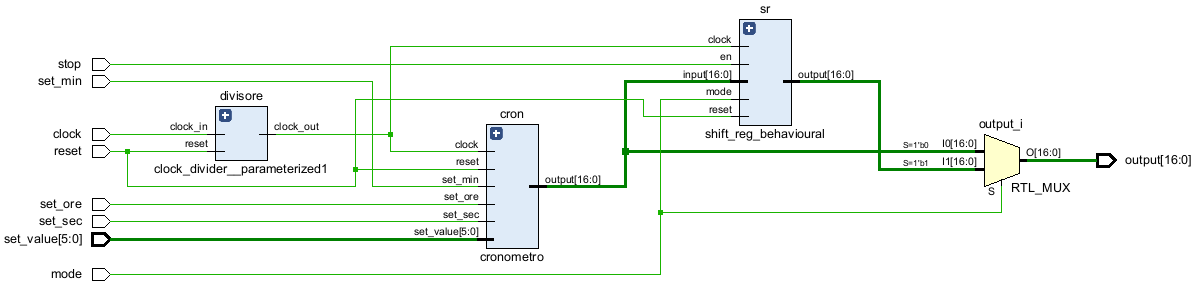
\includegraphics[width=17cm]{immagini/esercizio5/schema_5.3.png}
    \caption{Schema Cronometro con Intertempo}
\end{figure}


È stato necessario però gestire la visualizzazione dell'output del sistema complessivo, in cui si deve scegliere se mostrare l'uscita del cronometro (tempo real-time) o quella del registro a scorrimento (intertempi). Per farlo è stata aggiunta un'assegnazione combinatoria, che cambia l'output a seconda della modalità:

Di seguito è mostrato il codice relativo al componente che ingloba gli altri e allo shift register modificato.

\begin{lstlisting} [language=VHDL, caption= Top]
library IEEE;
use IEEE.STD_LOGIC_1164.ALL;

entity top is
    Port (
        set_value: in std_logic_vector (5 downto 0);
        set_sec,set_min,set_ore,mode,stop: in std_logic;
        reset: in std_logic;
        clock: in std_logic;
        output: out std_logic_vector (16 downto 0)
    );
end top;

architecture Structural of top is

    component shift_reg_behavioural is
        Port (
            input: in std_logic_vector (16 downto 0);
            clock,en: in std_logic ;
            reset,mode: in std_logic ;--mode 0: scrittura, mode 1: lettura
            output: out std_logic_vector (16 downto 0)
        );
    end component shift_reg_behavioural;

    component  cronometro is
        Port (
            set_value: in std_logic_vector (5 downto 0);
            set_sec,set_min,set_ore: in std_logic;
            reset: in std_logic;
            clock: in std_logic;
            output: out std_logic_vector (16 downto 0)
        );
    end component cronometro;
    component clock_divider is
        generic(
            clock_frequency_in : integer := 100000000;--100MHz
            clock_frequency_out : integer := 10000000 --10 MHz
        );
        Port ( clock_in : in  STD_LOGIC;
             reset : in STD_LOGIC;
             clock_out : out  STD_LOGIC);
    end component;

    signal cron_out,shift_out: std_logic_vector (16 downto 0);
    signal s_clk:std_logic ;

begin

    cron: cronometro 
        port map(
            set_value=> set_value,
            set_sec=>set_sec,
            set_min=>set_min,
            set_ore=>set_ore,
            reset=>reset,
            clock=>s_clk,
            output =>cron_out
        );

    sr: shift_reg_behavioural 
        port map(
            input=>cron_out,
            en=> stop,
            mode=> mode,
            reset=>reset,
            clock=>s_clk,
            output=>shift_out
        );


    divisore: clock_divider
        port map(
            clock_in=>clock,
            reset=>reset,
            clock_out=>s_clk
        );
    with mode select output <=
        cron_out  when '0',
        shift_out when '1',
        cron_out when others;

end Structural;


\end{lstlisting}


\begin{lstlisting} [language=VHDL, caption= Shift Register]
library IEEE;
use IEEE.STD_LOGIC_1164.ALL;

entity shift_reg_behavioural is
    Port (
        input: in std_logic_vector (16 downto 0);
        clock,en: in std_logic ;
        reset,mode: in std_logic ; --mode 0 : scrittura, mode 1: lettura
        output: out std_logic_vector (16 downto 0)
    );
end shift_reg_behavioural;

architecture Behavioral of shift_reg_behavioural is

   signal s1,s2,s3,s4: std_logic_vector (16 downto 0):="00000000000000000";

begin

    process (clock)
    begin
        if (falling_edge (clock)) then
        
            if ( reset='1') then
                s1<="00000000000000000";
                s2<="00000000000000000";
                s3<="00000000000000000";
                s4<="00000000000000000";
            
            elsif (mode='0' and en='1') then
                s1<=input;
                s2<=s1;
                s3<=s2;
                s4<=s3;
                
            elsif (mode ='1'and en='1') then
                s1<=s4;
                s2<=s1;
                s3<=s2;
                s4<=s3;
            end if;
        end if;
    end process;

    output<= s4;

end Behavioral;
\end{lstlisting}


\subsection{Testing}
È stato effettuato unicamente il test dell'unità top, essendo stati già precedentemente testati tutti gli altri componenti. In primo luogo, è stato effettuato il reset della macchina e successivamente sono stati mandati i segnali di stop per memorizzare gli intertempi. In particolare, sono stati memorizzati 4 intertempi e successivamente sono stati visionati in maniera circolare per 3 volte.

\begin{lstlisting} [language=VHDL, caption= Shift Register]
library IEEE;
use IEEE.STD_LOGIC_1164.ALL;

entity top_tb is
end top_tb;

architecture Behavioral of top_tb is

component top is
Port (
        set_value: in std_logic_vector (5 downto 0 );
        set_sec,set_min,set_ore,mode,stop: in std_logic;
        reset: in std_logic;
        clock: in std_logic;
        output: out std_logic_vector (16 downto 0 )
    );
end component top;

signal s_set_sec, s_set_min, s_set_ore, s_reset, s_clock, s_mode, s_stop: std_logic  := '0';
signal s_output: std_logic_vector(16 downto 0 ) :=  (others => '0');
signal s_set_value: std_logic_vector(5 downto 0 ) :=  (others => '0');
constant clk_period: time := 1 ns;

begin
   dut: top
    port map (
        set_value => s_set_value,
        set_sec=> s_set_sec,
        set_min=> s_set_min,
        set_ore=> s_set_ore,
        reset=> s_reset,
        clock => s_clock,
        output => s_output,
        mode=> s_mode,
        stop=>s_stop
    );
    
    tb: process
    begin
            wait for 100ns;
            s_reset <= '1';
            wait for 10ns;
            s_reset <= '0';
            
            wait for 50ns;
            s_stop<='1';
            wait for 10*clk_period;
            s_stop<='0';
            wait for 10ns;
            s_stop<='1';
            wait for 10*clk_period;
            s_stop<='0';
            wait for 30ns;
            s_stop<='1';
            wait for 10*clk_period;
            s_stop<='0';
            wait for 10ns;
            s_stop<='1';
            wait for 10*clk_period;
            s_stop<='0';
            
            wait for 50ns;
            s_mode<='1';
            wait for 10*clk_period;
            s_stop<='1';
            wait for 10*clk_period;
            s_stop<='0';
            wait for 10*clk_period;
            s_stop<='1';
            wait for 10*clk_period;
            s_stop<='0';
            wait for 10*clk_period;
            s_stop<='1';
            wait for 10*clk_period;
            s_stop<='0';
            wait for clk_period ;
            wait;
    end process tb;
    
    clock: process
    begin
        s_clock <= '1';
        wait for clk_period/2;
        s_clock <= '0';
        wait for clk_period/2;
    end process clock;
end Behavioral;
\end{lstlisting}